%!TEX root = mb.tex

\section{Evaluation} \label{sec:eval}

As we showed in \S\ref{sec:impl}, \sys supports all middlebox applications in typical outsourcing environments~\cite{aplomb,nfv} -- including header-only middleboxes (which \sys supports without modification) as well as DPI middleboxes (which \sys supports with modifications to their codebase). 
Hence, from a functionality perspective, \sys answers our original question, ``Is it possible to enable a third party to perform traffic processing for an enterprise, {\em without seeing the enterprise's traffic}?''  strongly in the affirmative.

To evaluate \sys more deeply, we now investigate whether \sys is practical from a performance perspective, looking at the overheads due to encryption and redirection. 
Overall, we find that \sys provides client performance comparable to APLOMB~\cite{aplomb} -- e.g., page load times increase by \todo{foo}\% relative to APLOMB when caching is disabled, and by \todo{bar\%} when caching is enabled.
\sys does impose some overhead at the gateway and middleboxes:
\sys with no DPI reduces gatway throughput by \todo{foo\%} and has zero overhead at the outsourced middleboxes. \sys with DPI enabled imposes a higher overhead, with the gateway throughput reduced by \todo{bar\%} and typical middlebox throughput reduced to \todo{baz\%} of baseline. 

\todo{methodology, datasets...}

\subsection{End-to-End Performance}
We first inspect end-to-end client performance when traffic is redirected through \sys.

{\it Does \sys provide web performance comparable to other outsourcing approaches?}
Page load times relative to APLOMB.

{\it How much does bandwidth increase between the gateway and the cloud from using \sys? How much would this bandwidth increase an enterprises networking costs?}



\subsection{Gateway Performance}
\begin{figure}[t]
  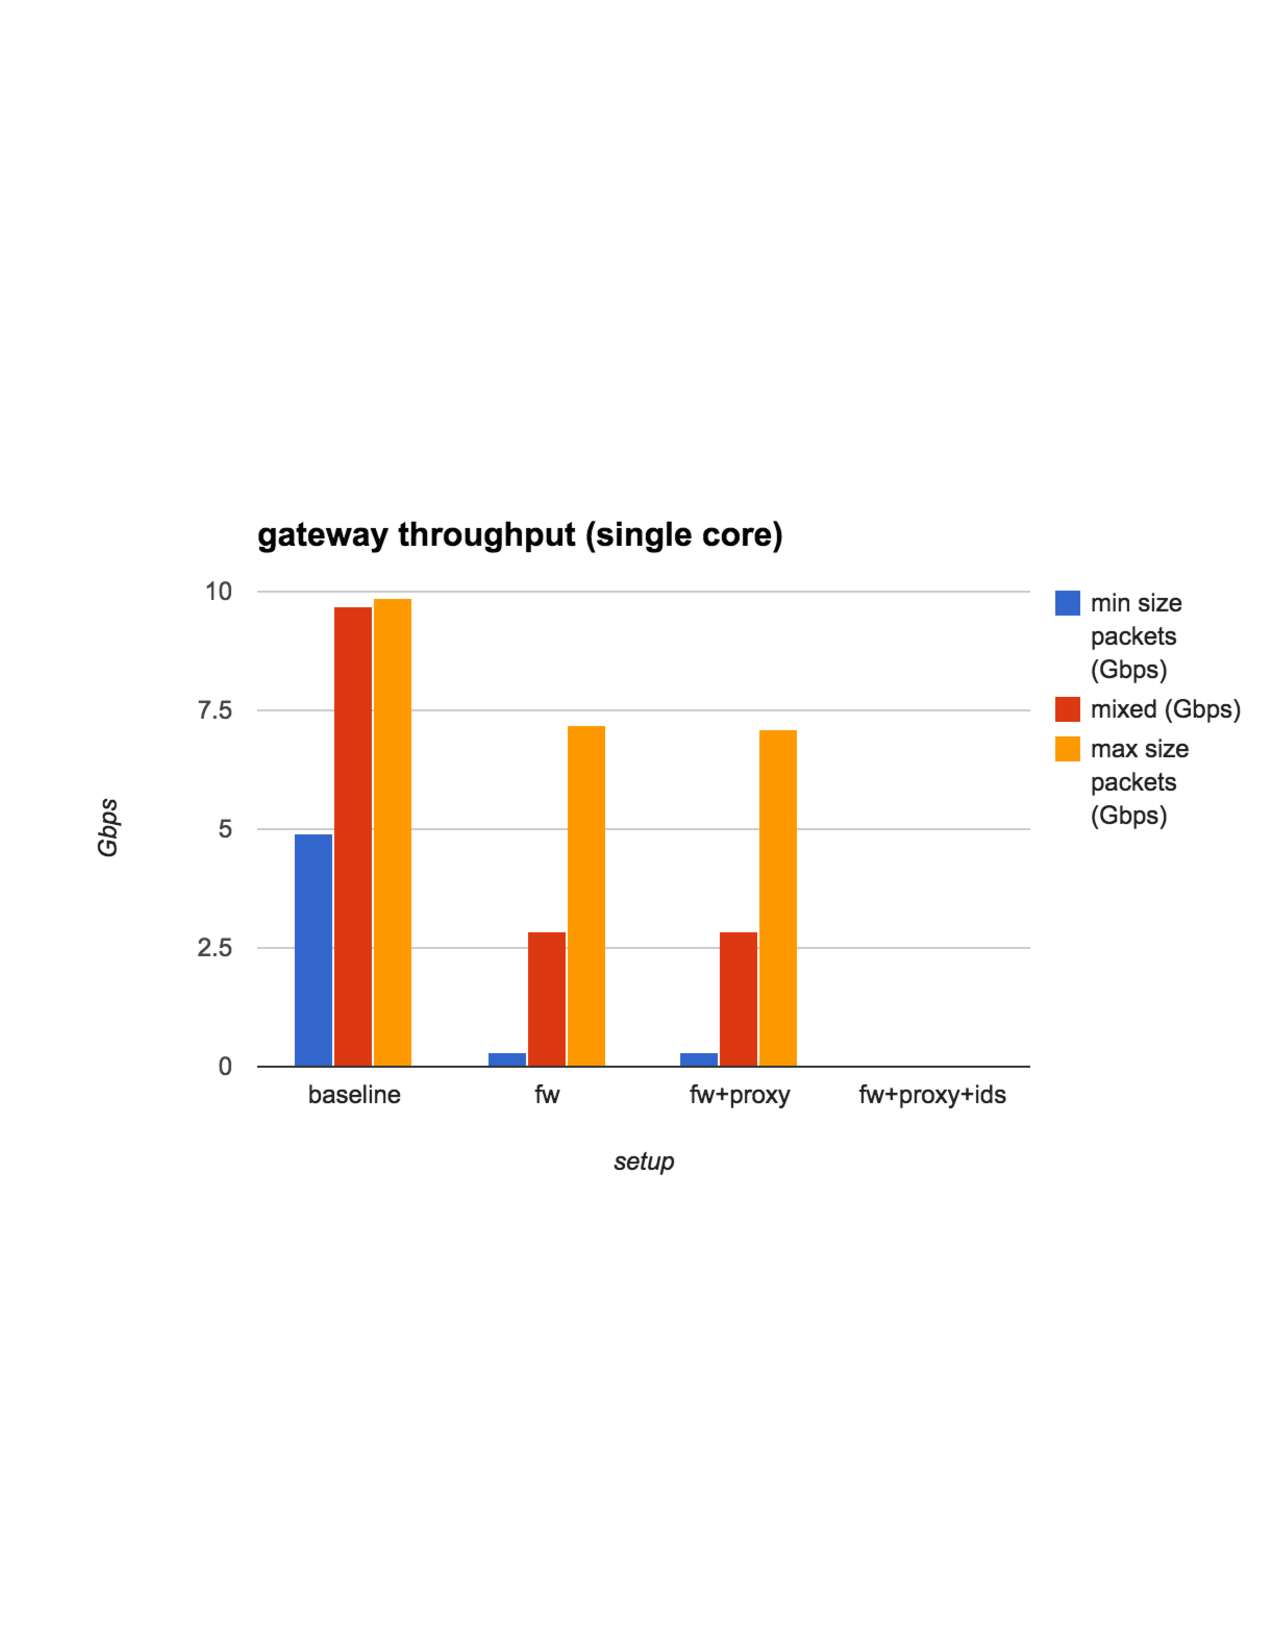
\includegraphics[width=3in]{fig/gatewayxput}
  \caption[]{\label{fig:gwxput} Throughput at the gateway without \sys, with header-only \sys, with HTTP-aware \sys, and with DPI-enabled \sys.}
\end{figure}


\noindent{\it How does encryption impact throughput at the outsourcing gateway relative to an outsourcing gateway without \sys?}
Figure~\ref{fig:gwxput}...

\begin{figure}[t]
  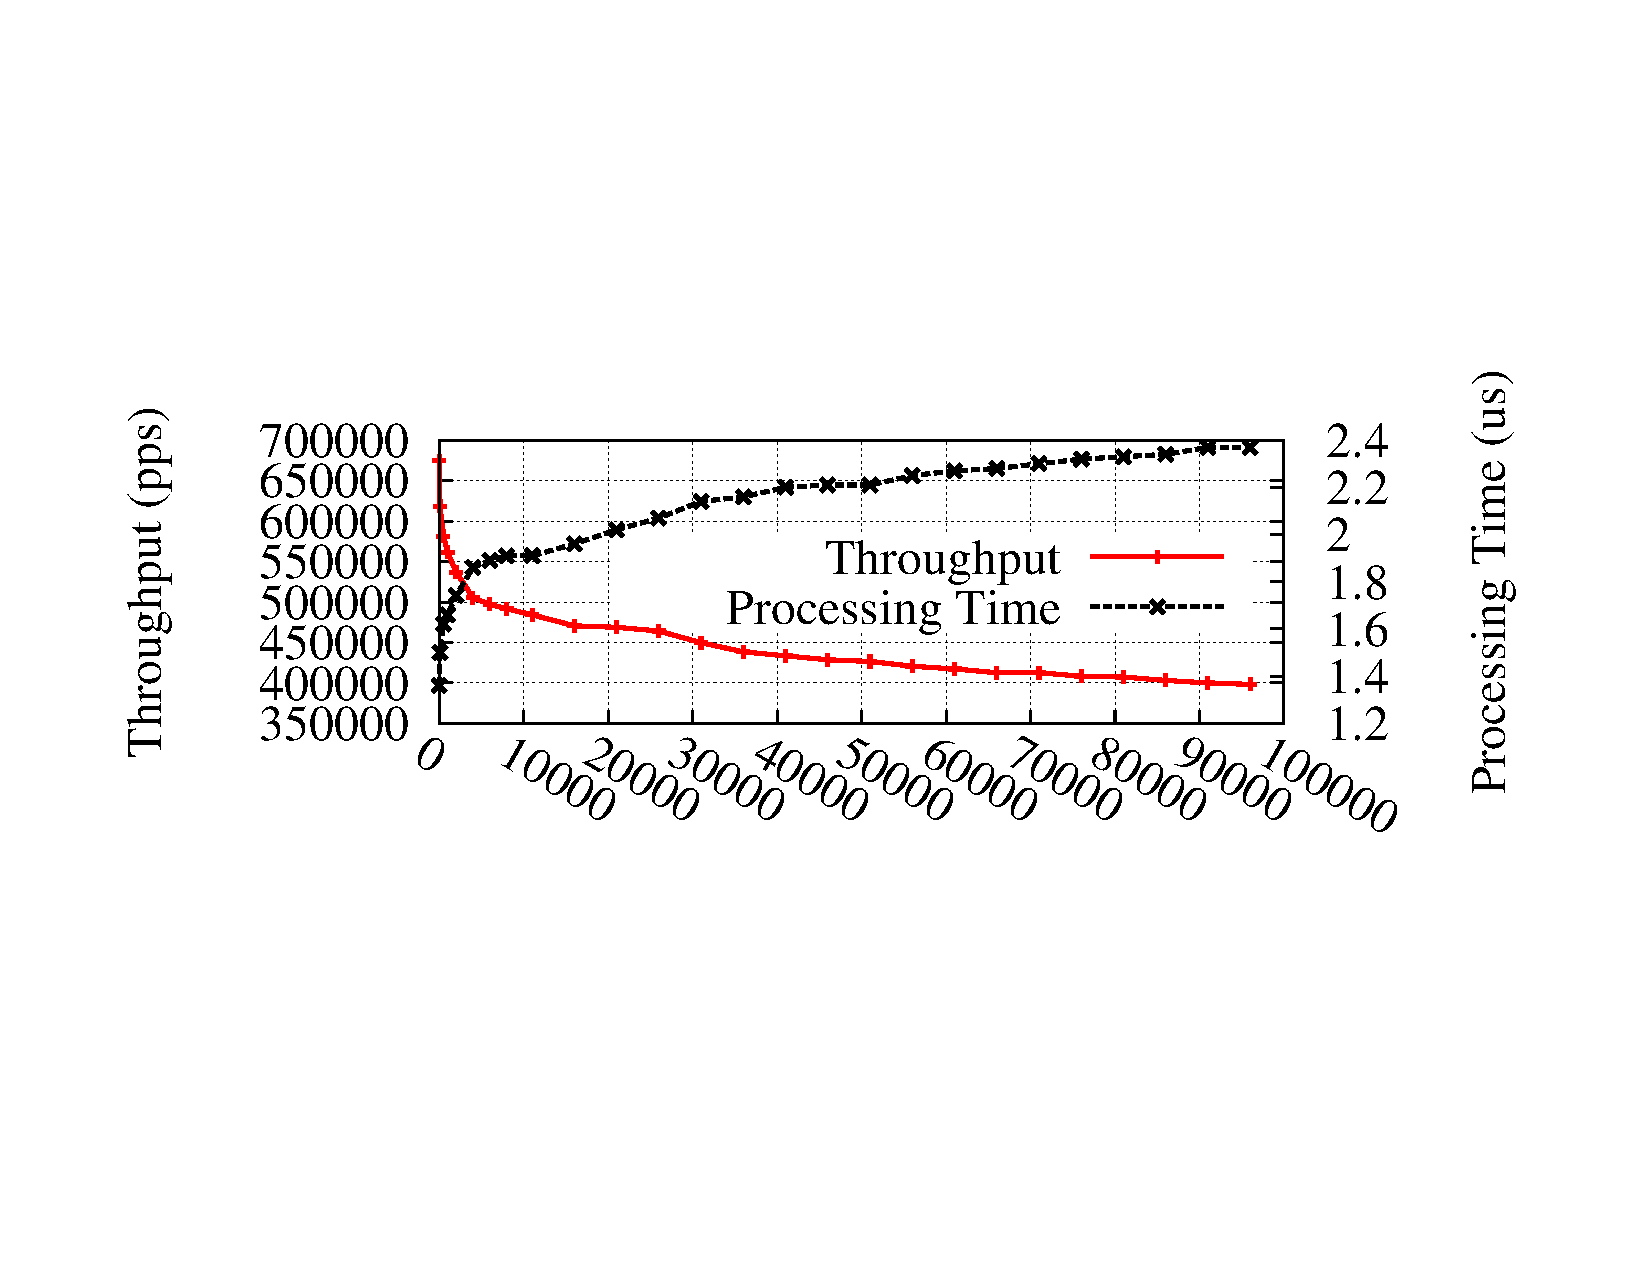
\includegraphics[width=3in]{fig/xputrange}
  \caption[]{\label{fig:xputrange} Throughput as number of rules for range encrypt increases.}
\end{figure}


\begin{figure}[t]
  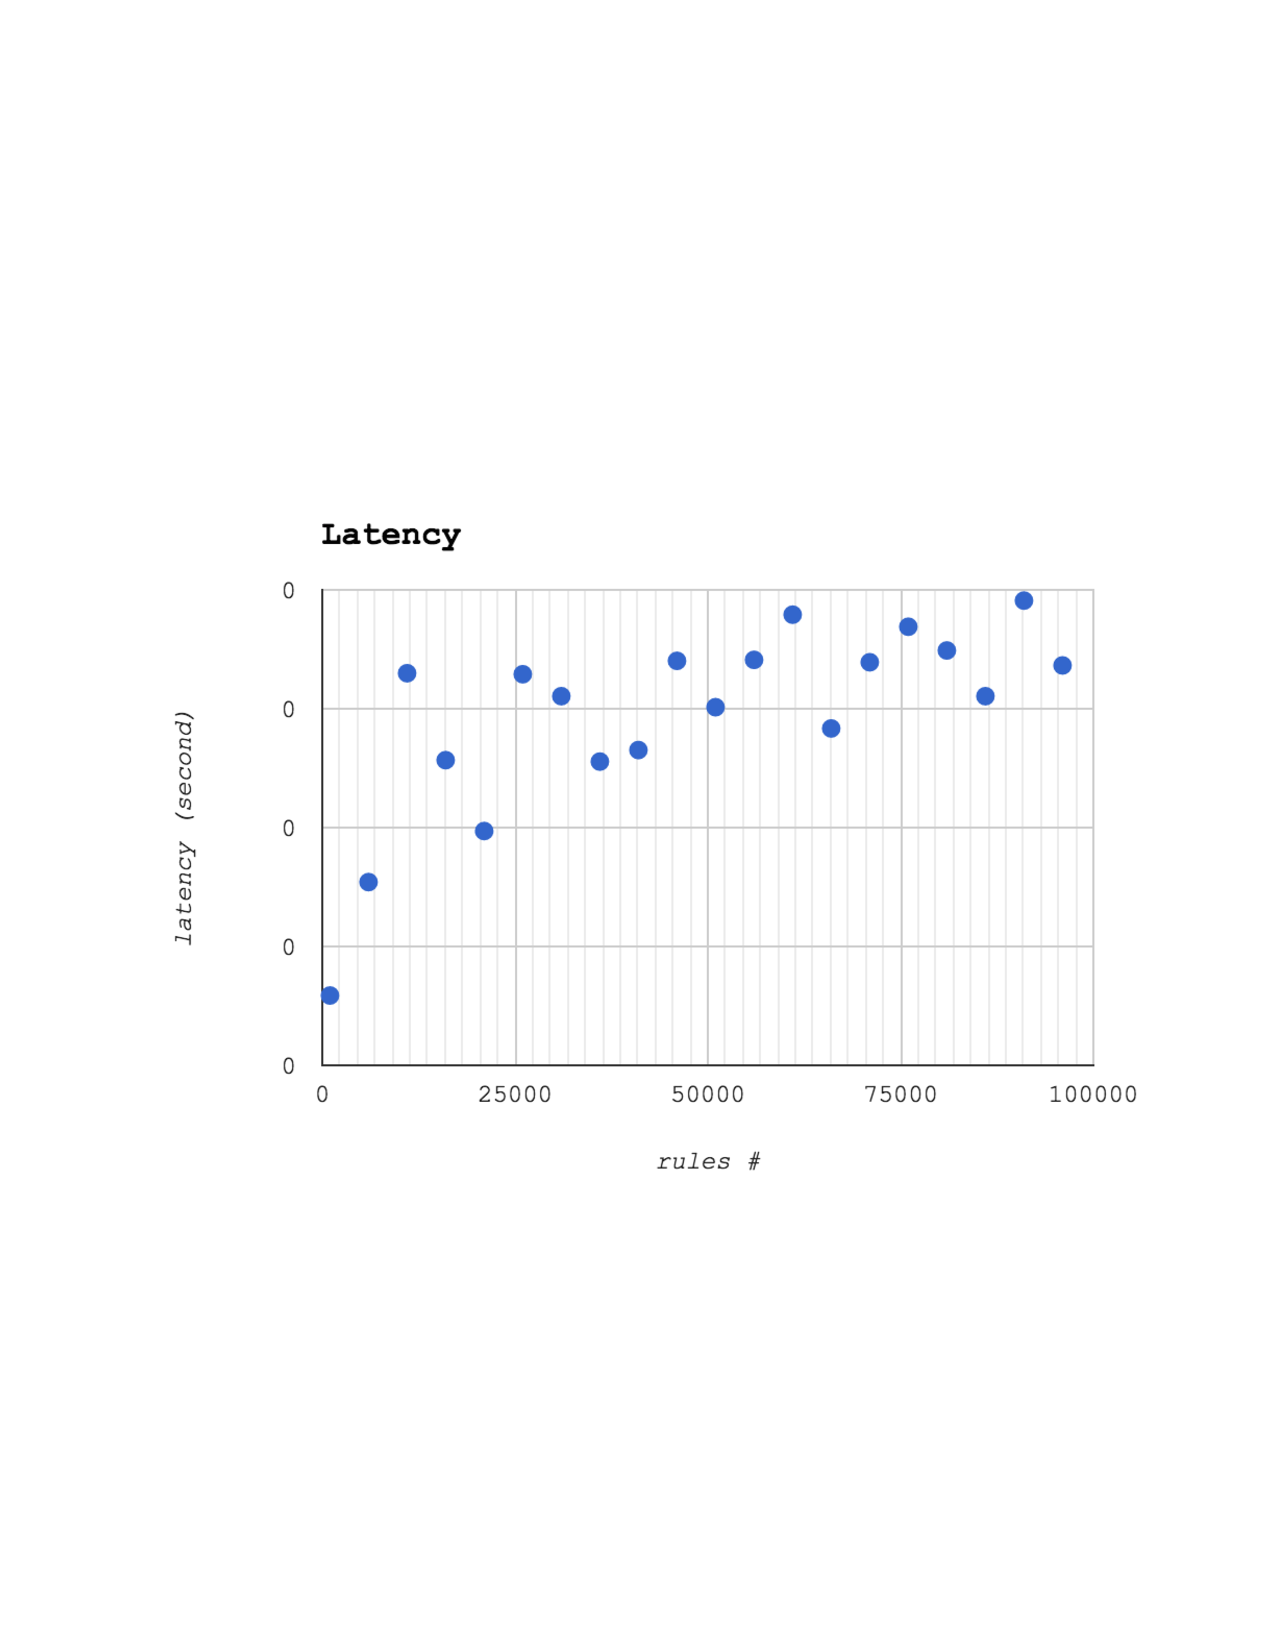
\includegraphics[width=3in]{fig/latencyrange}
  \caption[]{\label{fig:latencyrange} Per-packet latency as number of rules for range encrypt increases.}
\end{figure}


\noindent{\it How do throughput and latency at the gateway scale with the number of rules for range encryption?} 
Figs~\ref{fig:latencyrange} and~\ref{fig:xputrange}

\noindent{\it What is the memory overhead of the stateful range map encryption scheme?}


\subsection{Middlebox Throughput}

\begin{table}[t!]
\begin{tabular}{p{2.5cm}|p{1.4cm}|p{2cm}|p{1cm}}
Application & Header / HTTP / DPI & Baseline xput & \sys xput \\
\hline \hline
IP Firewall &   &  &  \\
Application Firewall & & & \\
NAT & Yes  & &  \\
IP Forwarding & & & \\
VPN Gateway &  &  &  \\ 
Load Balancer L4 & & & \\
Load Balancer L7 & & & \\
WAN optimizer  & & & \\
Web proxy/cache forward/ reverse & & &\\
IDS & & & \\
Exfiltration/parental filtering & & &  \\
\todo{split this} 
\end{tabular}
\caption{Middlebox applications supported by \sys and their throughput with an emprical traffic workload. \label{tbl:appsxput}}
\end{table}

\noindent{\it Is throughput reduced at the middleboxes due to \sys?}
(Hopefully we can say, for most apps, not at all)
Table~\ref{tbl:appsxput}...


\subsection{Header-Only Middleboxes}


\noindent{\bf Firewalls.} {\it Does \sys support all rules in a typical firewall configuration? How much does the ruleset ``expand'' due to encryption?}

\noindent{\it How often do updates to the firewall require a rule refresh? How long does it take to refresh rules at the firewall?}

\noindent{\bf NAT.}
\noindent{\bf LB...}

\subsection{DPI Middleboxes}

\noindent{\bf Proxy/Caching.}
{\it How many active connections per second can the Proxy accept? How does this compare to an unencrypted Proxy implementation, like Squid?}

{\it What improvement in page load times does a client experience due to proxying, relative to no proxy at all? Relative to an unencrypted proxy implementation?}

\noindent{\bf Intrusion Detection}
{\it How much does MBArk reduce flow completion times relative to BlindBox~\cite{blindbox}?}

\begin{table}[h]
\centering
\begin{tabular}{l|l|l|l|l}
&MBArk&APLOMB&BlindBox&SSL\\
\hline
\hline
Handshake&&&&\\
\hline
Total FCT&&&&\\
\end{tabular}

\end{table}

\noindent{\it What fraction of IDS rules can be supported without requiring decryption?}
Table, Zhi's stuff.
